\documentclass[11pt]{article}

\title{Building 3D Dense Reconstructions using LiDAR from a Walking Robot}
\author{Marcelo Gennari do Nascimento \\ Wadham College, University of Oxford}
\date{\today}

\usepackage{geometry}
 \geometry{
 a4paper,
 left=20mm,
 right=20mm,
 bottom=20mm,
 top=20mm,
 }
 
\setlength{\headheight}{14pt} 
\usepackage{setspace}
\usepackage{graphicx}
\usepackage{sidecap}

\usepackage[labelfont=bf]{caption}
\usepackage{amsmath}
\graphicspath{ {images/}}
\doublespacing

\begin{document}
	\pagenumbering{gobble}

	\maketitle

	\newpage

	\begin{abstract}
		Abstract text goes here.
	\end{abstract}

	\newpage
	\tableofcontents

	\newpage
	\pagenumbering{arabic}
	\section{Introduction}
	\paragraph{}
	Autonomous robots are going to be one of the major achievements of science to the benefit of the public. Autonomy though depends on two main problems that are tightly related to each other: Localization and Mapping. The first concerns the problem of localizaing a robot in an environment given a map as a prior. The second concerns the problem of mapping the environment given a prior robot's trajectory. Most of the time though, neither the trajectory nor the map is known a priori, and they need to be built simultaneously.
	
	\paragraph{}
	Since the 1986 IEEE Robotics and Automation Conference, researchers have framed the general problem of Simultaneous Localization and Mapping (SLAM) as the ``holy grail" of modern robotics \cite{SLAMPartI}. A reliable solution to this problem would make autonomy one step closer to reality. Since the conference, a number of algorithms have been developed that successfully tackle SLAM, each of them with their advantages and drawbacks. Modern methods of localization are able to predict the position of a walking robot to up to 2cm \cite{7041346}.
	
	\paragraph{}
	In order to make the map built have significant meaning and be of use to people, it is necessary to reconstruct it in 3D (or volumetrically). A 3D reconstruction system would give geometric, semantic and graphical meaning to maps, which then can be used for augmented or virtual reality.
	
	\paragraph{}
	Volumetric reconstruction relies heavily on tracking the robot's position, since the observation accuracy is independent from other observations but bounded by the tracking accuracy. Therefore, by using modern techniques to solve the problem of SLAM, it would be possible to build a reliable and realistic map of an environment without any prior information about how the environment is structured. Obvious direct applications for such a system would be reconaissance, search and rescue, and transportation.
	
	\subsection{Aim of the Project}
	\paragraph{}
	This project is concerned with putting together state of the art algorithms for SLAM and reconstruction systems to reliably and effiiciently build a 3D map of an environment with LiDAR data from a walking robot without any prior map or trajectory available. 
	
	\paragraph{}
	Even though many papers have been published in the individual building blocks that form the components of this project, it is harder to find academic reports that put all of the state of the art algorithms together to form a working system.
	
	\subsection{ Organisation of the Report}
		\paragraph{Section 2} of the report will go through the literature review of the main building blocks of the project. In particular, we will explore the current developments in the solutions of the Simultaneous Localization and Mapping (SLAM), the Iterative Closest Points (ICP) and 3D Reconstruction problem.
		
		\paragraph{Section 3} will go deeper on the system pipeline of the project. In order to get a general understanding of the system, detaied explanation of the steps of data processing, inputting and outputting will be explained. This will also introduce the two main parts of the system that will be explained in subsequent sections.
		
		\paragraph{Section 4} explores the solution of the SLAM problem adopted in the project. Since building an accurate map is an essential step to the success of the project, this section will explain the details of how the SLAM solution works and why this particular structure was chosen.
		
		\paragraph{Section 5} shows how the output from the SLAM solution will be integrated with the 3D reconstruction system.
		
		\paragraph{Section 6} will conclude the report with an overall evaluation of how the system performed. It will also indicate ways in which the system could be improved in a subsequent project. An analysis of how the outcome of this project compares with similar systems will be provided.

	\newpage
	\section{Literature Review}
	\subsection{Simultaneous Localization and Mapping (SLAM)}
	\paragraph{}
	SLAM is the problem of whether it is possible for a mobile robot to create a globally consistent map of an environment and localize itself on it without prior knowledge of the map \cite{SLAMPartI}\cite{Cadena}. Building a map of an environment is a crucial step towards autonomy, since planning and control assume prior knowledge of mapping and localization. Mathematically, we can frame SLAM as a Markov Chain, a Bayes Net or a Factor Graph. Defining:
	
	\begin{itemize}
		\item $\mathbf{x_k}$: the pose of the robot (being $\mathbf{X_{0:k}}$ as the poses from time $\mathbf{0}$ to $\mathbf{k}$)
		\item $\mathbf{u_k}$: the odometry measurement ($\mathbf{U_{0:k}}$ as the historical measurements)
		\item $\mathbf{l_k}$: the landmark observation ($\mathbf{L_{0:k}}$ as the historical landmarks)
		\item $\mathbf{c_k}$: the loop closures
	\end{itemize}

	It is possible to formulate the problem of SLAM more formally using both a factor graph or a probabilistic framework:

	\begin{figure}[h]
		\centering
		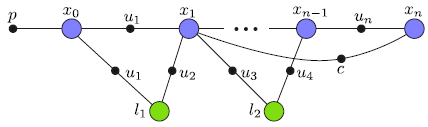
\includegraphics{SLAMFactorGraph.png}
		\caption{SLAM as a Factor Graph. The value $\mathbf{p}$ denotes a prior; $\mathbf{x_n}$ denotes the state vector; $\mathbf{u_n}$ denotes odometry measurements; $\mathbf{c}$ denotes close loops; $\mathbf{l_n}$ denotes landmark positions.}
		\label{fig:slam1}
	\end{figure}
	
	\paragraph{}
	The graph shown in Figure \ref{fig:slam1} is a Factor Graph representation of the dependencies between variables and measurements. A probabilistic framework can then be extracted from it. 
	\begin{equation}
	P(X,L,U,Z)\ \propto \ P(x_0)\prod_{i=1}^{M}P(x_i|x_{i-1}, u_i)\prod_{k=1}^{K}P(z_k|x_{i_k},l_{j_k})
	\label{probSLAMeq}
	\end{equation}
	\paragraph{}
	The general goal of probabilistic SLAM is to find variables $\mathbf{X^*}$ and $\mathbf{L^*}$ that maximizes the posterior probability distribution $P(X,L\ |\ U, Z)$ of the Equation \ref{probSLAMeq}. Two models of the probabilities given above are used commonly in SLAM to tackle this problem: the Process Model (also known as Motion Model in mobile robotics) and Observation Model:
	
	\begin{minipage}{.5\linewidth}
		\centering
		\begin{equation*}
		\begin{split}
		\mathbf{Process\ Model:} \\ 
		x_i = f(x_{i-1}, u_i) + w_i
		\end{split}
		\end{equation*}
	\end{minipage}
	\begin{minipage}{.5\linewidth}
		\centering
		\begin{equation*}
		\begin{split}
		\mathbf{Observation\ Model:} \\ 
		z_i = h(x_{i_k}, l_{j_k}) + v_k
		\end{split}
		\end{equation*}
	\end{minipage}
	
	\paragraph{}
	where $w_i$ is white noise with covariance $Q$ and $v_k$ is white noise with covariance $R$. The process (motion) model is usually a generalization of how the robot moves (kinematics) \cite{Montemerlo02fastslam:a}\cite{772544}. The observation model is a probabilistic representation of the performance of the sensors used to collect the data. Notice that both models are probabilistic and thus define the probabilitiy distributions $p(x_i|x_{i-1},u_i)$ and $p(z_k|x_{i_k},l_{j_k})$.

	\paragraph{}
	Under this framework, the mathematical analysis of SLAM has been shown that it is indeed feasible to build a nondivergent map with no prior information, so it is widely accepted that in theoretical grounds, SLAM is a solved problem \cite{SLAMPartI}\cite{Cadena}\cite{CsorbaThesis}\cite{938381}. However, there are computational and algorithmic challenges that hinders the development of a real-time implementation system that performs SLAM. This problem gets even more complicated when considering unstructured environments and large scale maps \cite{SLAMPartII}.
	
	\paragraph{}
	There are three main implementations of SLAM: Kalman Filtering and Extended Kalman Filtering (with early works such as proposed by R. Smith \cite{Smith:1990:EUS:93002.93291}), Particle Filtering (most notably with FastSLAM \cite{Montemerlo02fastslam:a}) and Information Filter (with the now state-of-the-art work of iSAM from Michael Kaess \cite{Kaess08tro}).

	\subsubsection{Kalman Filtering}
	\paragraph{}
	As one of the first implementations to appear to solve the problem of SLAM, the Extended Kalman Filtering (EKF) approach makes two approximations when formulating the probabilistic SLAM: both the Process Model and the Observation Model are linearized about a suitable linearization point $\hat{x}$.

	\paragraph{}
	 Subsequently, the probability distributions $p(x_i|x_{i-1}, u_i)$ and $p(z_i|x_i, l_i)$ are modeled as Gaussians with the mean as $\nabla f|_{x=\hat{x}}$ and $\nabla h|_{x=\hat{x}}$ and covariances $Q$ and $R$. With this framework in place, a recursive two-step method can be found to update the posterior probability distribution at every iteration \cite{SLAMPartI}:
		\begin{equation*}
		\mathbf{Prediction\ Phase:}\ \ 
		P(x_{i},L|Z_{0:i-1}, U_{0:i}) = \int P(x_i | x_{i-1}, u_{i}) P(x_{i-1}, L |Z_{0:i-1}, U_{0:i-1})dx_{i-1}
		\end{equation*}
		\begin{equation*}
		\mathbf{Update\ Phase:} \ \  P(x_i, L | Z, U) = \frac{P(x_{i}, L | Z_{i-1}, U)P(z_i|x_i,L)}{P(z_i|Z, U)}
		\end{equation*}	 	
	\paragraph{}
	The Prediction Phase concerns the motion model, where an update of the estimated position of the mobile robot is made taking into account only the controls and kinematics of the robot itself. This is followed by an Update Phase, where the position of the robot is recalculated based oan the observation of a landmark, for example. This algorithm is then recursively applied for every time-step $i$. 	
	\paragraph{}	 
	 Since the product of two gaussians is a gaussian, the probability density function $p(x_i, L|Z, U)$ will remain Gaussian at all times, and a closed loop solution using just the mean and the covariance matrices can be found \cite{772544}.
	\paragraph{}	
	 Analysis of the EKF algorithms have shown that due to linearization of the functions $f$ and $h$, assumptions about Gaussian Process and Observation Model can cause the EKF solution to perform poorly unless many loop closures are detected in frequent intervals \cite{doi:10.1177/1729881416669482}.


	\paragraph{}
	It is also known that the Kalman Filter approach requires storage of the order of $O(N^2)$ (where $N$ is the number of features), and for a classic implementation of the algorithm, it also requires computational power of the order of $O(N^2)$ \cite{CsorbaThesis}. New methods for computing the covariances (which cause the squared dependence) by exploring state augmentation, partitioned updates and sparsity in the matrices have demonstrated faster solutions, thus requiring less computational power \cite{SLAMPartII}.

	\subsubsection{Particle Filtering}
	\paragraph{} 
	In order to avoid linearlization of nonlinear models, Particle Filtering (PF) has been a popular method to integrate non-gaussian distributions in the estimation \cite{Montemerlo02fastslam:a}\cite{772544}. The basis of particle filtering comes from Dallert's proposal of a Monte Carlo Localization (MCL) algorithm \cite{772544}. In sampling methods, the probability distributions are defined in function of the density of particles along the distribution. This approach avoids the assumption of linearity and Gaussian distribution, which makes this algorithm embrace multi-modal distributions.
	
	\paragraph{}
	Just like the EKF solution, there are many ramifications of PF methods. However, most of them follow the basic structure of the FastSLAM algorithm \cite{Montemerlo02fastslam:a}. This algorithm breaks the SLAM problem in one of localization over the robot's path, and $k$ of landmark location, where $k$ is the number of landmarks. The Localization problem is solved using MCL, which is composed of two parts \cite{772544}:
	 
	 \paragraph{Prediction Phase:} In this part, $N$ number of particles are drawn from the Motion Model distribution, whose density asymptotically represents the proposal distribution $P(X, L | Z_{0:i-1}, U)$.
	 
	 \paragraph{Update Phase:} Each particle from the Prediction Phase is then given a weight which is equal to the likelihood of the particle being there given the observation. In other words, $weight = P(Z|X, L)$, which is drawn from the Observation Model.
	 
	 \paragraph{}
	 After those two phases, the Landmark Location is solved using the classical EKF algorithm.
	 
	 \paragraph{}
	 Particle filtering methods have advantage over the EKF for not making any assumptions about linearity or Gaussianity of the distribution. Also if implemented wisely, it can reach $O(Mlog(K))$ time, where $M$ is the number of particles and $K$ is the number of landmarks \cite{Montemerlo02fastslam:a}.
	 
	 
	
	\subsubsection{Information Filter}
	\paragraph{}
	Information Matrices formulations of the SLAM algorithm is a technique used to compensate the quadratic dependency in computation time of the EKF by exploiting the sparsity in the Information Matrix.
	\paragraph{}
	It is known that the Dense Covariance Matrix in the EKF is the key to a convergent solution \cite{SLAMPartI}. However, this dense matrix means that the EKF will need computational power increasing quadratically in the number of landmarks.
	
	\paragraph{}
	By adopting an information matrix formulation of the EKF (the Information Matrix is defined as the inverse of the covariance matrix, or equivalently the coefficient matrix of the least square problem), this can be reduced for constant time computation \cite{doi:10.1117/12.381658}. This formulation is exactly equivalent to the EKF, with the advantage of being computationally advantageous \cite{Dellaert-2006-9639}.
	
	\paragraph{}
	The Information Filtering and Information Smoothing approaches have had many ramifications (with special mention to the Sparse Extended Information Filter (SEIF)\cite{doi:10.1117/12.381658}. The main algorithm that was developed was the iSAM (Incremental Smoothing and Mapping) \cite{Kaess08tro}.
	
	\paragraph{}
	By tracking the information filter, which is naturally sparse, iSAM captures the structure of the SLAM system in a compact, memory and computationally light way.
	
	[explain about $|Ax-B|_2$ and the sparsity in the Information Matrix = $A^TA$]
	
	\subsection{Iterative Closest Points (ICP)}
	\subsection{Stereo Visual Odometry}
	\subsection{3D Reconstruction Systems}

	\newpage
	\section{System Pipeline} \label{pipeline}
	\paragraph{}
	The pipeline for the overall system can be seen below. It consists of 4 modules: (I) First odometry estimates (based on either Visual Odometry or Wheel Odometry); (II) Laser Odometry (using Simona Nobili's AICP \cite{7989547}); (III) Loop closure detection and Graph Optimization (using iSAM \cite{Kaess08tro}); (IV) 3D dense volumetric reconstruction (using BOR\textsuperscript{2}G-CUBES \cite{TannerFSR2015}\cite{TannerArXiv2016}).

	\paragraph{}
	These 4 modules are broken down in two parts: the first part is concerned about solving the SLAM problem, which outputs a reliable trajectory and map. The second part is concerned about inputting that to a 3D reconstruction system (which in this case if BOR\textsuperscript{2}G-CUBES) to build the environment volumetrically.

	\newpage
	\section{SLAM Solution}
	\paragraph{}
	As already introduced in Section \ref{pipeline}, the SLAM solution has 4 independent building blocks. This offers flexibility enough to test the effect that each part has in the outcome of the map. This section is going to discuss deeper how the solution works with all the building blocks working together. 
	 
	\subsection{First Odometry Measurements}
	\paragraph{}
	The first odometry measurements offer a relatively inaccurate estimation of the pose of the robot at a certain time. It is used as the input pose to the AICP algorithm in order for it to process laser odometry based on the LiDAR scan.
	
	\paragraph{}
	During the project, two mehods to get the first odometry measurements were used. When getting data with the mobile robot Husky \cite{Husky}, the wheel odometry provided by the system served as a good first estimate of its position. When getting the data with the MultiSense SL \cite{multisense}, Stereo Visual Odometry from MultiSense's stereo camera was performed to get the first odometry estimations.
	\subsubsection*{Wheel Odometry}
	\paragraph{}
	Remember to put the pictures of the Wheel Odometry and the corrected pose using AICP.
	\subsubsection*{Stereo Visual Odometry}
	\paragraph{}
	The Stereo Visual Odometry used is based on the system described at \cite{VisualOdometry} and implemented as the fovis library \cite{fovis}.
	\paragraph{}
	Remember to put the pictures of the Visual Odometry and the corrected pose using AICP. 
	\paragraph{}
	Also a good idea would be to put the Wheel Odometry and the Visual Odometry as comparison using the same Dataset (the one that Simona Collected at Edinburgh would be perfect)
		
	\paragraph{}
	IMAGES
	
	
	
	
	\subsection{Laser Odometry}
	\paragraph{}
	Given the first odometry measurements, the AICP algorithm was used to incorporate the LiDAR scan of each of the paths to the estimation problem. For the Husky example, the Velodyne \cite{velodyne} LiDAR was used, whereas for the Oxford Dataset, the MultiSense SL LiDAR was used.
	
	\paragraph{}
	The results for each of the paths are shown below for comparison. It is noticeable the difference between the accuracy of the First Odometry Measurements to the Laser Odometry. However, it can be seen that there is drift due to how the AICP algorithm works.
	
	\subsection{Loop Closure Detection}
	\paragraph{}
	In order to adjust for the innacuracies of the path estimate, a loop closure detection algorithm was placed. Since it was assumed that the robot would not overdrift, three simple heuristics were used to detect loop closure: Time Filter Sampling, Euclidean Distance, and Pose Alignment. 
	\begin{itemize}
		\item \textbf{Filter Sampling:} In order to avoid the problem of loop closing two state estimates that are in the same room but did not leave the room, a time filter sampling was applied. The idea is to sample every $S$ state estimates, so that the candidate loop closing states would be sparse enough so that the loop just occurs between big time frames, but dense enough to apply euclidean distance.
		\item \textbf{Euclidean Distance:} Once the estimates have been  sampled, the euclidean distance between each of them is applied. If the distance between any two states is less than a threshold value $E$, then the two estimates form a candidate pair and they are added in the candidate pair list.
		\item \textbf{Pose Alignment:} After the resampling, the candidates pairs are tested for their relative pose. Since the loop closure correction relies on alignment of point clouds using ICP, it is a good strategy to select poses that would maximize the overlap between the point clouds associated with the candidates. In order to do that, another resampling is done based on the overlap between the field of view of the estimates. If the overlap is less than a threshold value $O$, then the candidate pair is dropped out from the list, and the remaining are the loop closures that are considered.
	\end{itemize}
	
	\paragraph{}
	The parameters $S$, $E$ and $O$ are chosen by hand depending on what dataset is used in the algorithm. Changing the parameters can affect the outcome of the map significantly, so it is important to spend some time tuning them to the specific requirements of the test.
	
	\paragraph{}
	Figure \ref{fig:loopClosureDetection} shows the results of the Loop Closure detection when applied to the Husky dataset. Due to the relatively low velocity of the mobile robot, the parameters were adjusted to match the time that the mobile robot would take to leave a room before coming back to the same room.
	\begin{SCfigure}
	\begin{minipage}{0.67\textwidth}
				\centering
				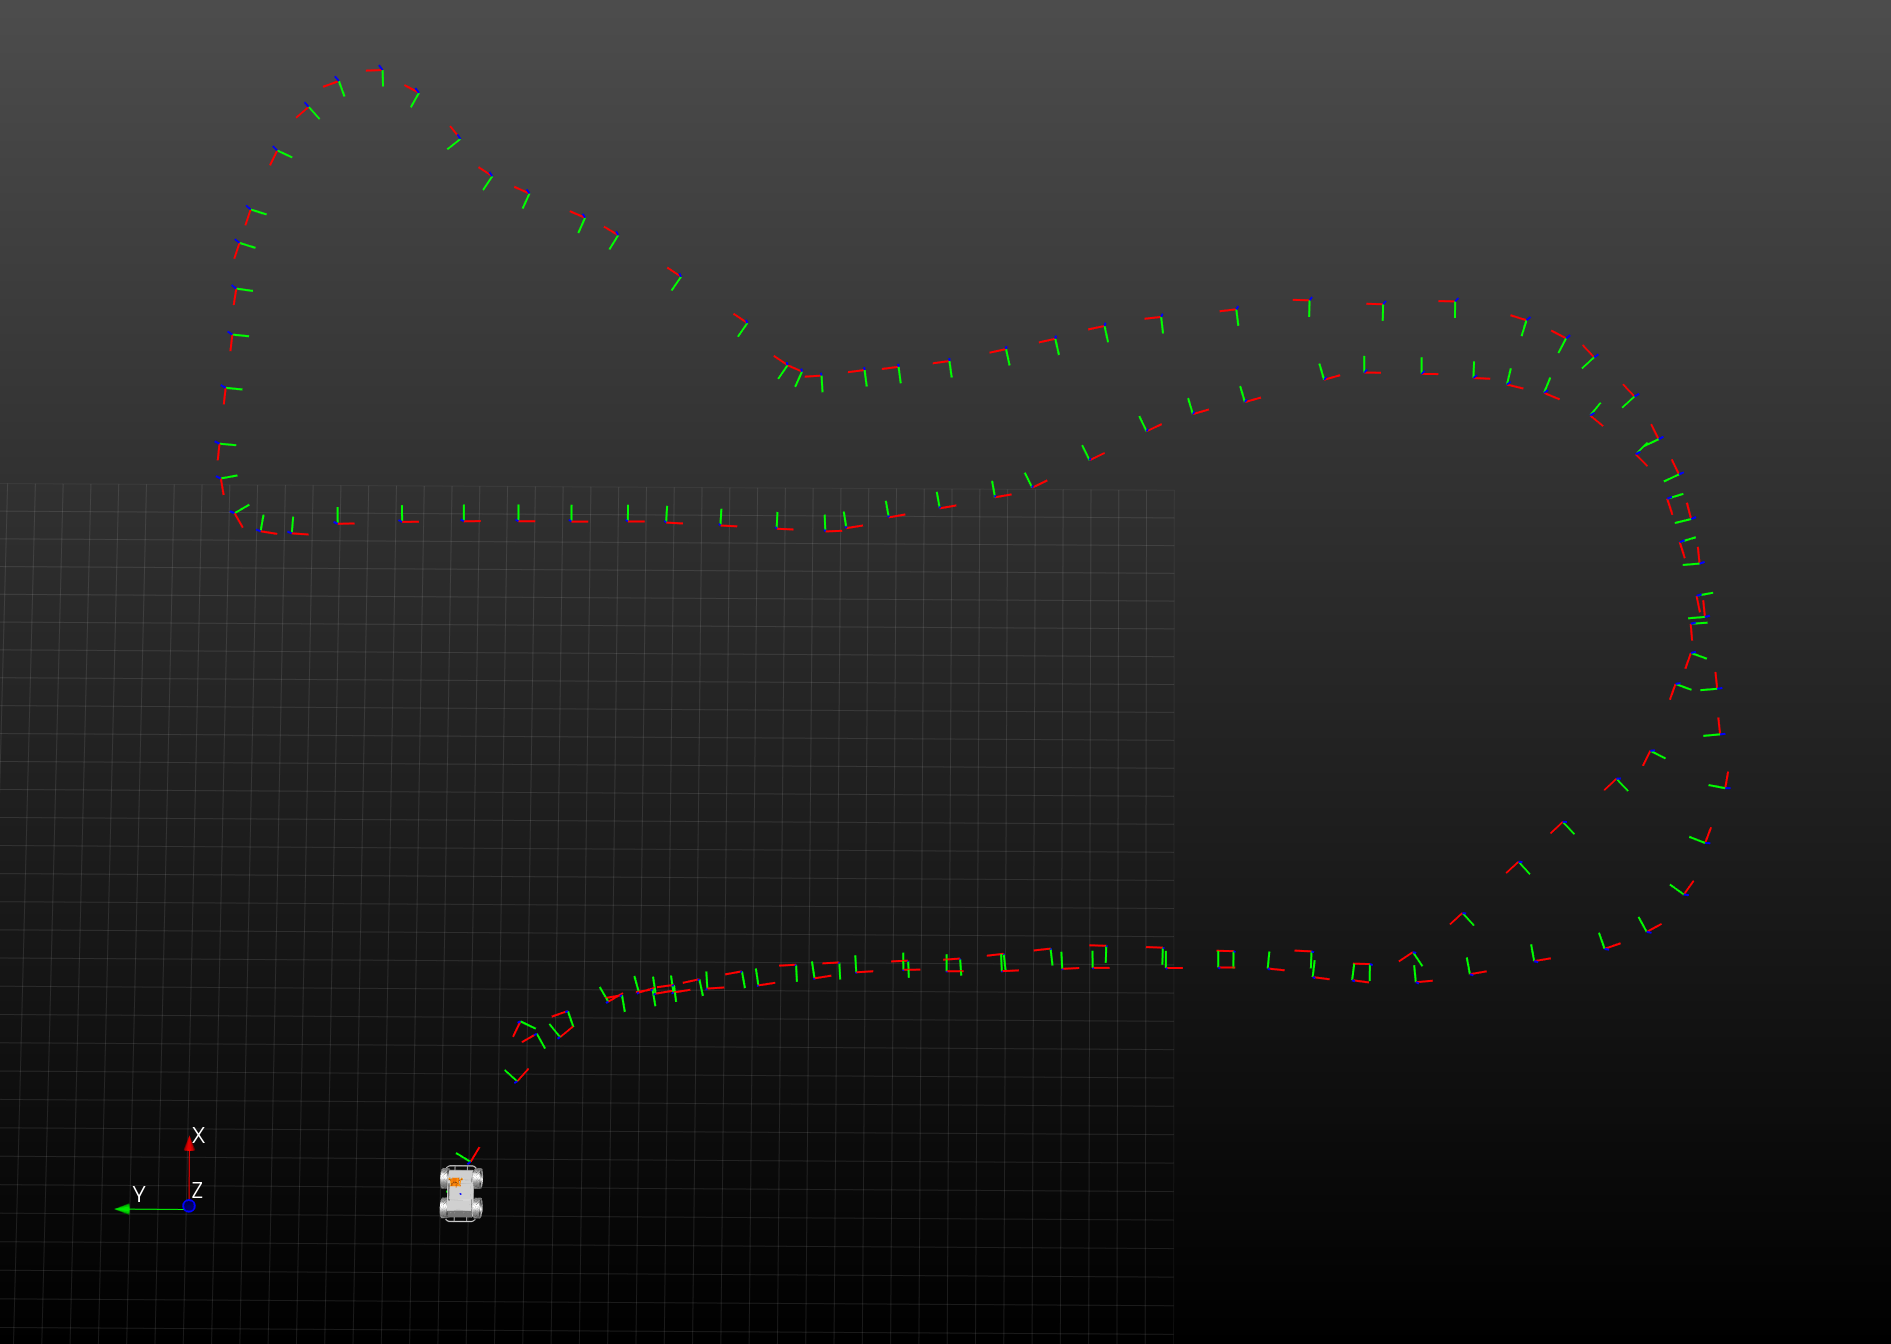
\includegraphics[width=\textwidth]{LoopClosureTimeSampling}
				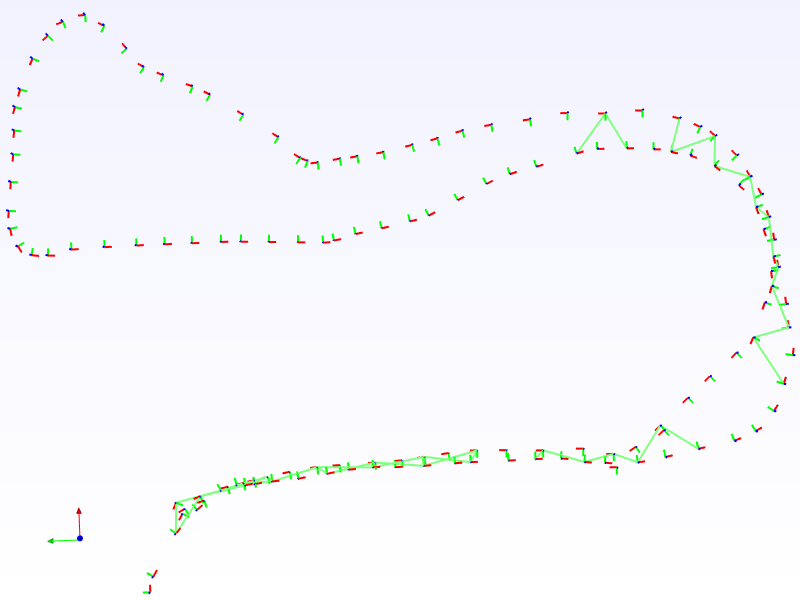
\includegraphics[width=\textwidth]{LoopClosureEuclideanSampling}
				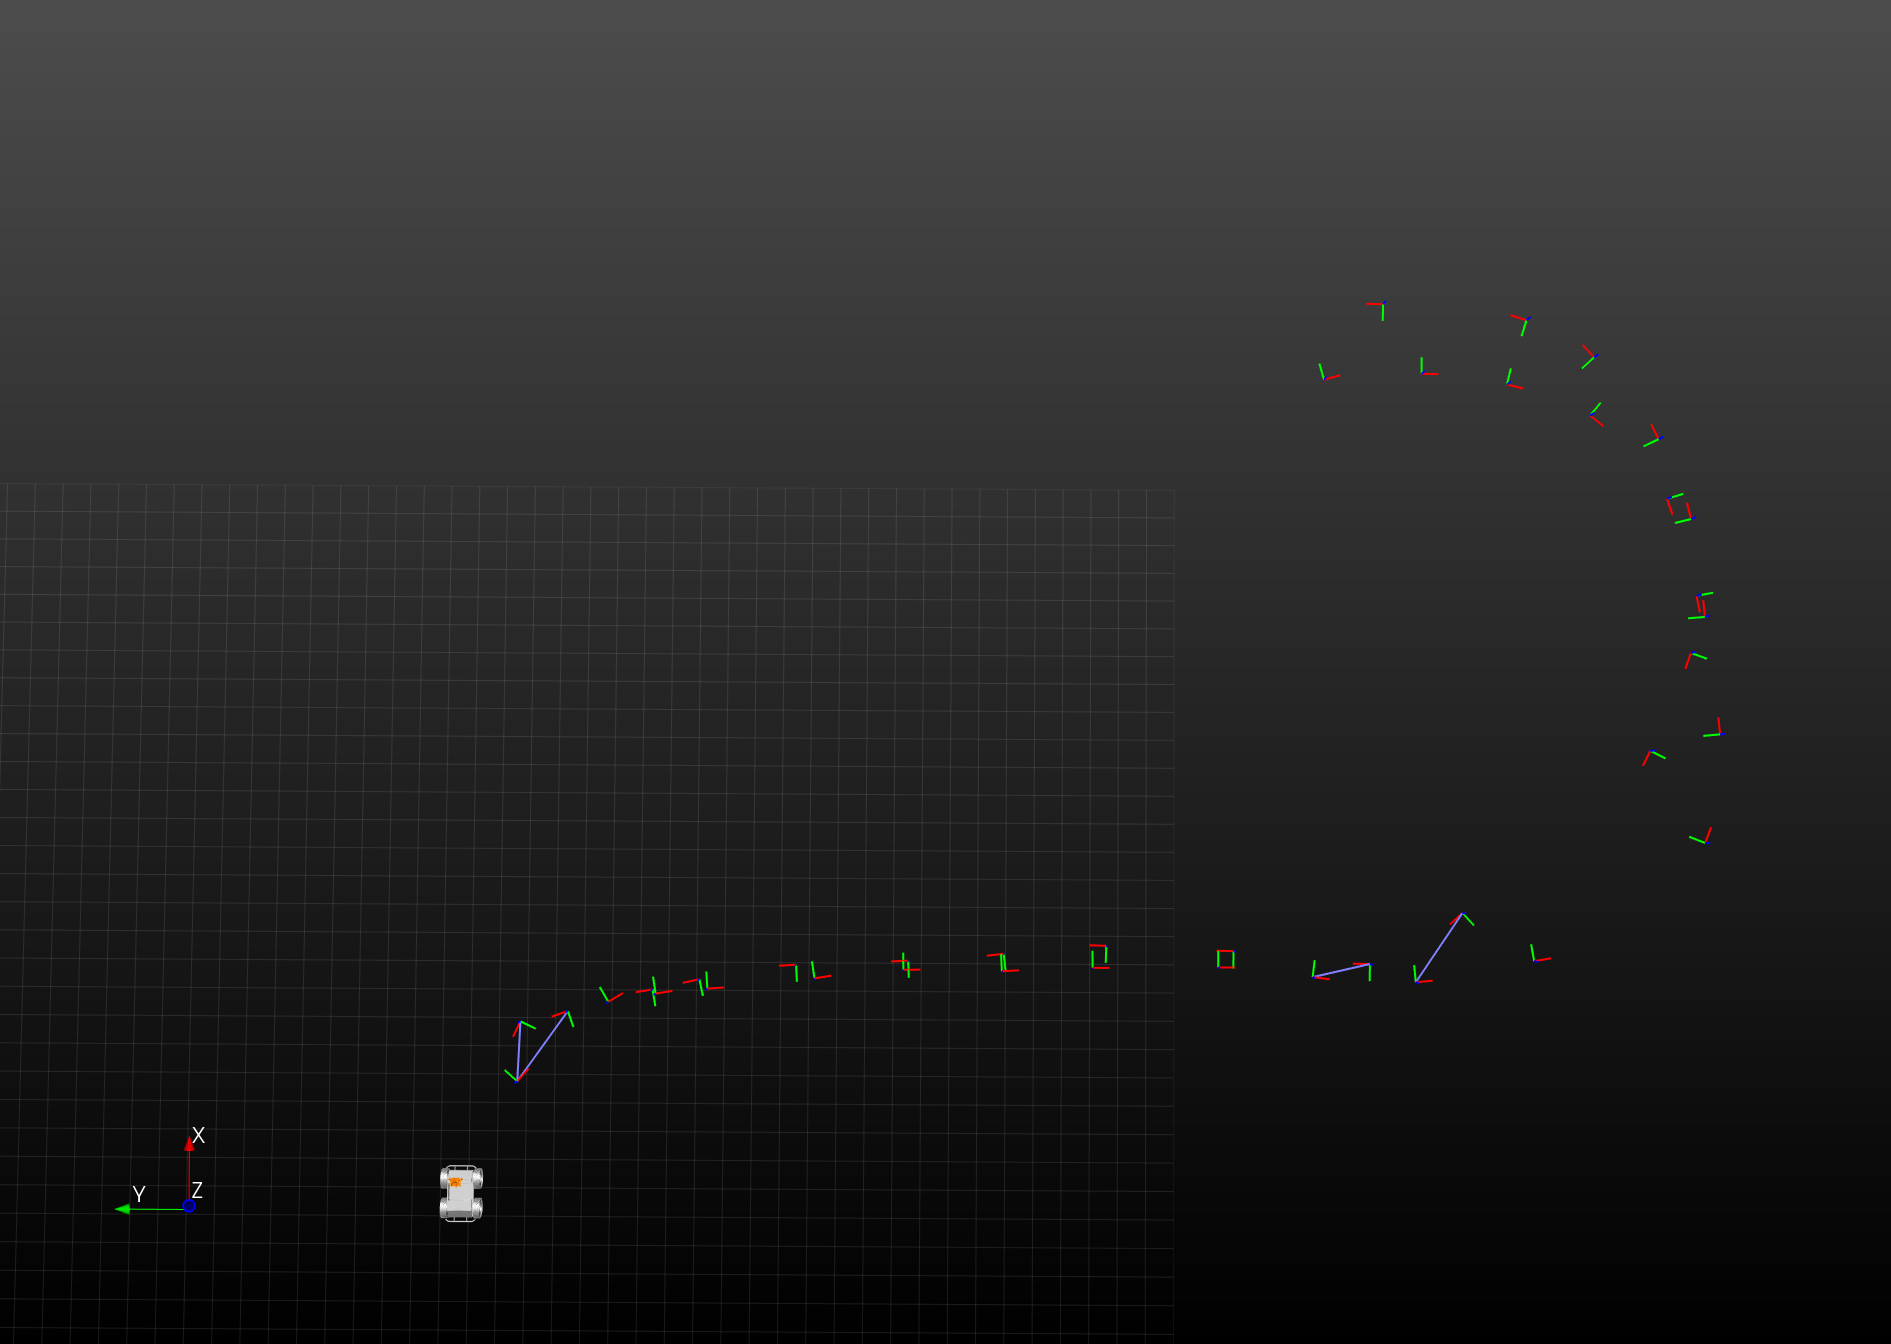
\includegraphics[width=\textwidth]{LoopClosureFinal}
	\end{minipage}\hfill
	\begin{minipage}{0.33\textwidth}
		\centering
		\caption[t]{The three heuristics for loop closure detection. Data shown was collected using the Husky Mobie Robot and the Velodyne LiDAR, visualized in bird's-eye view with red and green coordinates representing the path of the robot. The figure on the top shows the result of the time sampling. The plot in the middle shows the Euclidean Distance Pairings. The last figure is the result of the Pose (overlap) filter. In this experiment, $S=2$, $E=2$ and $O=0.5$.}
		\label{fig:loopClosureDetection}
	\end{minipage}
	\end{SCfigure}
	\paragraph{}
	It is also important to notice that marginally different parameters have an impact on the number of loop closures and on the outcome of the map. Figure X shows the results of different maps according to different settings of the loop closure parameters.
	
	\paragraph{}
	Ideally, the number of loop closures should be neither too big nor too small. Loop closure can be thought of strings "tightening" the Factor Graph in Figure \ref{fig:slam1} by adding constraints to it. If many loop closures are made, the graph becomes to constraint and new corrections to the map would be insignificant. This can be naively desirable since it means that the certainty of the graph is high, but if one loop closure is a bit off, then the effect cannot be corrected subsequently. In the other hand, if few loop closures are made, then the drift between poses are not corrected substantially and the overall error in the graph is high.
	
	\paragraph{}
	Therefore it is crucial to tune the parameters so that meaningful loop closures are selected. 

	\subsection{Graph Optimization}

	\newpage
	\section{Integration with BOR\textsuperscript{2}G-CUBES}
	
	\newpage
	\section{Conclusion}

	\newpage
	\bibliography{4YPReportBibl}
	\bibliographystyle{ieeetr}

\end{document}
